\subsection{UC4 - Selezione manuale delle Features}
\label{uc4}

    \begin{figure}[htbp]
        \centering
        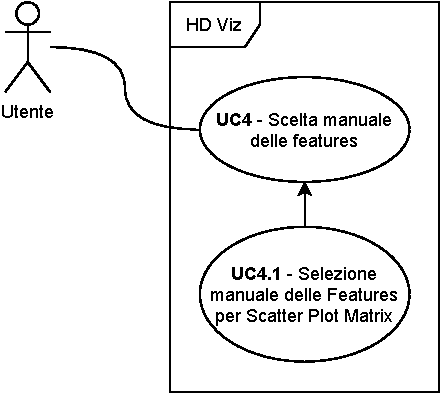
\includegraphics[width=0.5\textwidth]{source/sections/casi-uso/diagrams/uc4.pdf}
        \caption{UC4 - Selezione manuale delle Features}
        \label{fig:uc4}
    \end{figure}
    
    \begin{itemize}
    \item \textbf{Attore}: utente;
    \item \textbf{Descrizione}: l'utente può scartare le features di un dato che non è interessato a visualizzare;
    \item \textbf{Precondizione}: 
     \begin{itemize}
        \item eseguito l'upload del dataset come matrice $N\times M$ (\hyperref[uc1]{UC1});
        \item Selezionato un tipo di visualizzazione (\hyperref[uc2]{UC2}).
    \end{itemize}
    \item \textbf{Postcondizione}: la matrice contiene $M-i$ colonne, dove $i$ è il numero di features che l'utente ha scartato;
    \item \textbf{Scenario Principale}: 
    \begin{enumerate}
        \item l'utente visualizza le features del dataset, che corrispondono alle colonne della matrice;
        \item l'utente scarta le features a cui non è interessato.
    \end{enumerate}
    \item \textbf{Generalizzazioni}:
        \begin{enumerate}
            \item selezione manuale delle features per Scatter Plot Matrix (\hyperref[uc4.1]{UC4.1}).
        \end{enumerate}
    \end{itemize}
    
    \subsubsection{UC4.1 - Selezione manuale delle Features per Scatter Plot Matrix}
    \label{uc4.1}
    \begin{itemize}
    \item \textbf{Attore}: utente;
    \item \textbf{Descrizione}: l'utente può selezionare al massimo 5 features da visualizzare;
    \item \textbf{Precondizione}: 
     \begin{itemize}
        \item eseguito l'upload del dataset come matrice $N\times M$ (\hyperref[uc1]{UC1});
        \item selezionato Scatter Plot Matrix come visualizzazione (\hyperref[uc2.1]{UC2.1}).
    \end{itemize}
    \item \textbf{Postcondizione}: la matrice contiene al massimo 5 colonne cioè le features che l'utente ha selezionato;
    \item \textbf{Scenario Principale}: 
    \begin{enumerate}
        \item l'utente visualizza le features del dataset, che corrispondono alle colonne della matrice;
        \item l'utente sceglie le features che è intenzionato a visualizzare.
    \end{enumerate}  
    \end{itemize}